\section{Parallel Directory Structure}

\begin{itemize}
\item {\tt BoxLib/} 

 BoxLib is a library for describing meshes consisting of a union
 of boxes.  The BoxLib modules define the basic datatypes used
 in Parallel.

\item {\tt docs/}

 Documentation describing BoxLib and other directories in Parallel.

\item {\tt mglib/}

  The C++ multigrid solver.

\item {\tt mk/}

  The generic Makefiles that store the compilation flags for
  various platforms.

\item {\tt scripts/}

  Some simple scripts that are useful for building, running,
  maintaining codes in Parallel.

\end{itemize}

\section{BoxLib Data Structures}

BoxLib contains the most fundamental objects used by applications written
in the Parallel directory; the objects in BoxLib support structured
grid adaptive mesh refinement (AMR), i.e. in a single calculation
different regions of the domain can have different spatial resolutions.  
At each level of refinement, the region covered by that level is broken
into boxes, or grids.  The entire computational domain is covered by
the coarsest (base) level of refinement, often called level 0. 
Higher levels of refinement have finer zones by a ``refinement ratio''
of either 2 or 4.  Only a portion of the domain may
be covered by the higher levels of refinement.  

The grids are properly nested, in the sense that the union of grids
at level $\ell+1$ is contained in the union of grids at level $\ell$.
Furthermore, the containment is strict in the sense that,
except at physical boundaries,
the level $\ell$ grids are large enough to guarantee that there is
a border at least $n_{\rm proper}$ level $\ell$ cells wide surrounding each level
$\ell +1$ grid (grids at all levels are allowed to extend to the physical
boundaries so the proper nesting is not strict there).
For parallel computations, the boxes are distributed to processors, in
a fashion designed to put roughly equal amounts of work on each
processor (load balancing).

On a grid, the data can be stored at cell-centers, on a face/edge, or
on the corners.  In BoxLib, data that is on an edge is termed `nodal'
in that direction (see Figure~\ref{fig:dataloc}).  Data that is on the
corners is nodal in all spatial directions.  In our Parallel applications, 
the state data (velocity, density, species $\ldots$) is generally
cell-centered.  Fluxes are nodal in the direction they represent.
A few quantities are nodal in all directions (e.g.\ the pressure in
the low Mach number projection methods).

\begin{figure}[h]
\centering
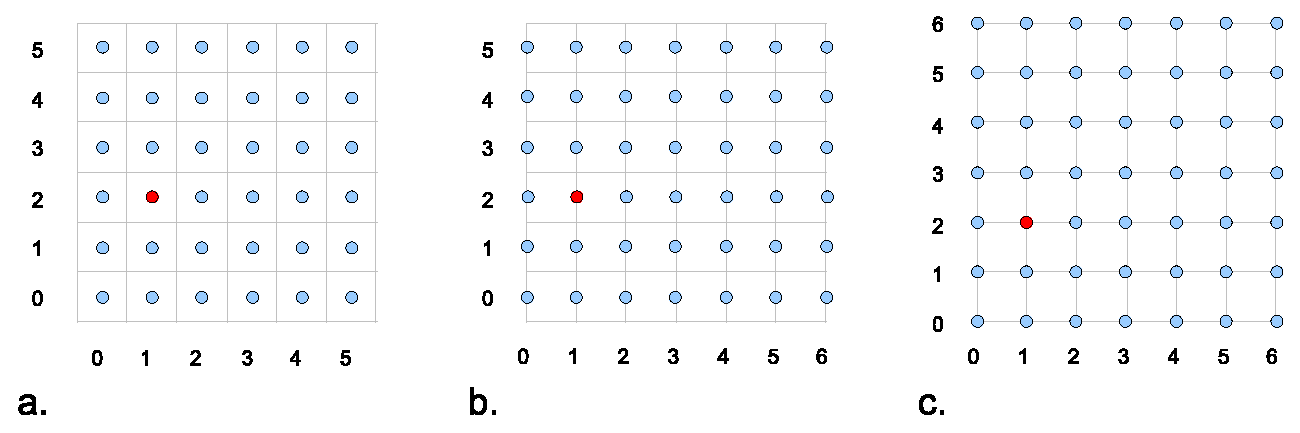
\includegraphics[width=6.5in]{\boxlibfigpath/data_loc2}
\caption[Data-centerings on the grid]
  {\label{fig:dataloc} Some of the different data-centerings:
  (a) cell-centered, (b) nodal in the $x$-direction, and (c) nodal in
  both the $x$- and $y$-directions.  Note that for nodal data, the
  integer index corresponds to the lower boundary in that direction.
  In each of these centerings, the red point has the same indices:\ (1,2).
  Not shown is the case where data is nodal in the $y$-direction only.}
\end{figure}

To simplify the description of the underlying AMR grid, BoxLib
provides a number of classes.  We briefly summarize some of the major
classes below.

First, note that when a Parallel application is compiled and linked,
the number of spatial dimensions (1,2 or 3), {\bf DIM},
 of the code must be specified.  The code that will be
built is specifically designed to run only with that number of dimensions.
(This is unlike the fParallel data structures in which we build
dimension-independent code at compile-time.)

\subsection{\IVtype}

\IVtype\s are n-tuples of integers that are used to define
indices in space.    An example of an \IVtype\ in 2D would
be (3,5).

\subsection{\Boxtype}

A \Boxtype\ is simply a rectangular domain in space.  Note that \Boxtype\s
do not hold any data themselves. A box basically contains
only the indices of its low end and high end as well as a type 
(cell-centered, edge-centered, or nodal).

\begin{figure}[h]
\centering
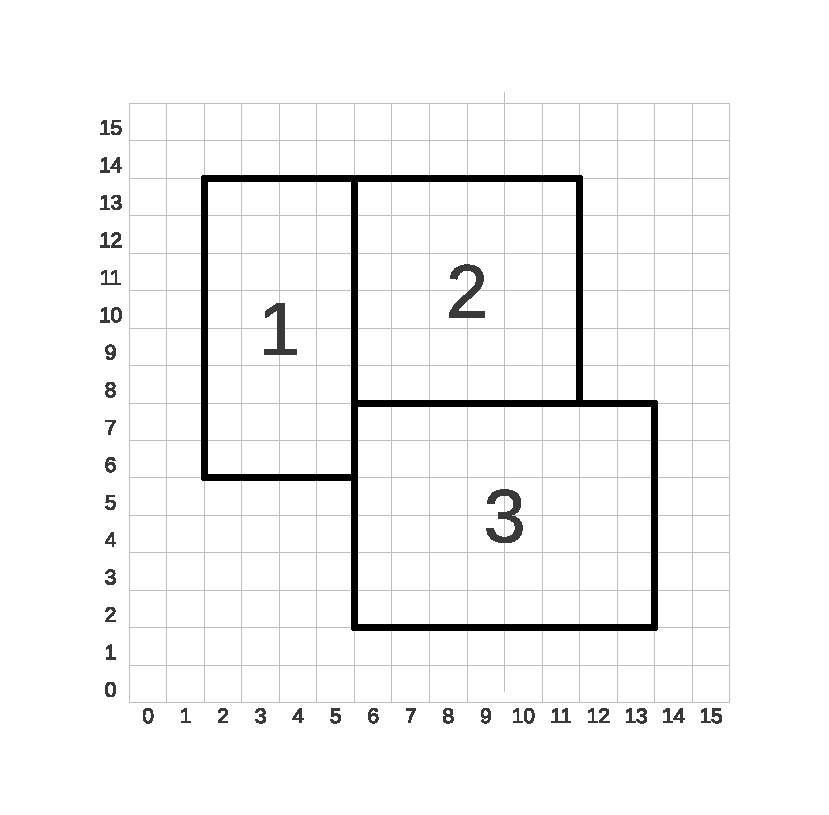
\includegraphics[width=4.0in]{\boxlibfigpath/index_grid2}
\caption[Single-level grid structure]
{\label{fig:boxes} Three boxes that comprise a single level.  At this
  resolution, the domain is 20$\times$18 zones.  Note that the
  indexing in BoxLib starts with $0$.}
\end{figure}

The computational domain is divided into boxes.  The collection of
boxes with the same resolution comprise a level.
Figure~\ref{fig:boxes} shows three boxes at the same level of
refinement.  The position of the boxes is with respect to a global
index space at that level.  For example, box 1 in the figure has 
{\tt lo} = (3,7) and {\tt hi} = (9,12).  

\subsubsection{Common Operations on a \Boxtype}

For a \Boxtype\ declared as:
\begin{verbatim}
  type(box) :: mybox
\end{verbatim}

You can access the indices of the boxes using the 

\begin{itemize}

\item {\tt smallEnd} 

\item {\tt hi = upb(mybox)} returns an array, {\tt hi(dm)}, with
     the box upper bounds

\end{itemize}

\subsection{\FAB}

A \FAB\ is a ``Fortran Array Box''.  It contains the state data in a
multidimensional array and several \Boxtype-types to describe where in
index-space it lives.  The datatype of a \FAB\ is
\begin{verbatim}
  type fab
     integer   :: dim = 0
     type(box) :: bx
     type(box) :: pbx
     type(box) :: ibx
     integer   :: nc = 1
     real(kind = dp_t), pointer, dimension(:,:,:,:) :: p => Null()
  end type fab
\end{verbatim}
 
\noindent Here:
\begin{itemize}
\item {\tt dim} is the dimensionality of the data
\item {\tt bx} is a \Boxtype\ describing the index space for which this \FAB\ is defined
\item {\tt ibx} is a \Boxtype\ that describes the index range of the valid data
  for the \FAB.  This differes from {\tt bx} when the box is nodal in one or more 
  directions.
\item {\tt pbx} is a \Boxtype\ that extends {\tt ibx} to include
  any ghostcells, or equivalently, the physical box for the \FAB\
\item {\tt nc} is the number of components (how many variables at  
  each grid location)
\item {\tt p} is a pointer to the data, in this case double precision
  ({\tt kind=dp\_t}).  Other \FAB\ types exists for other Fortran
  data types.
\end{itemize}


Note that all state data is stored in a four-dimensional array,
{\tt (nx,ny,nz,nc)} in size, regardless of the dimensionality of the
problem.  For 2D problems, {\tt nz=1}.

In Parallel, we don't usually deal with \FAB s alone, but rather
through \MultiFab s, described next.

\subsection{\MultiFab}

A \MultiFab\ is a collection of \FAB s at the same level of
refinement.  The data type of a \MultiFab\ is:
\begin{verbatim}
  type multifab
     integer :: dim = 0
     integer :: nboxes = 0
     integer :: nc = 1
     integer :: ng = 0
     logical, pointer :: nodal(:) => Null()
     type(layout) :: la
     type(fab), pointer :: fbs(:) => Null()
  end type multifab
\end{verbatim}

\subsection{\BoxArray}

A \BoxArray\ is an array of boxes.  

\subsection{\layout}

A \layout\ is basically a \BoxArray\ that knows information about other
boxes, or box ``connectivity.''  It contains additional information
that is used in filling ghost cells from other fine grids or from
coarser grids.  This information is stored as long as the layout
exists so that we don't have to recompute intersections every time we
do some operation with two MultiFabs that have that layout, for
example.
